\documentclass[tikz,border=4pt]{standalone}
\usepackage{amsmath,amssymb}
\usetikzlibrary{arrows.meta,calc}
\begin{document}
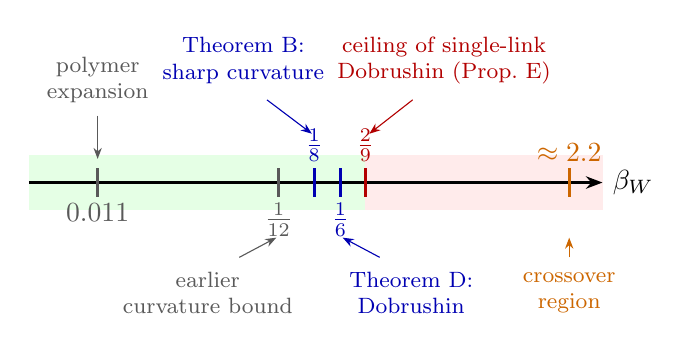
\begin{tikzpicture}[scale=1]
% log scale for beta_W (SU(2), d=4): x = 2.2*log10(beta_W)+6.6
\def\X#1{({2.6*log10(#1)+6.0})}
\fill[green!10] ({2.6*log10(0.005)+6.0},-0.35) rectangle ({2.6*log10(0.2222)+6.0},0.35);
\fill[red!8] ({2.6*log10(0.2222)+6.0},-0.35) rectangle ({2.6*log10(3.2)+6.0},0.35);
\draw[-{Stealth[length=6pt]},thick] ({2.6*log10(0.005)+6.0},0)--({2.6*log10(3.2)+6.0},0) node[right]{$\beta_W$};
\foreach \v/\lab/\pos/\col in {0.0109/{$0.011$}/below/gray!70!black, 0.08333/{$\tfrac1{12}$}/below/gray!70!black, 0.125/{$\tfrac18$}/above/blue!70!black, 0.16667/{$\tfrac16$}/below/blue!70!black, 0.22222/{$\tfrac29$}/above/red!70!black}
  {\draw[\col,line width=1.2pt] ({2.6*log10(\v)+6.0},-0.18)--({2.6*log10(\v)+6.0},0.18);
   \node[\pos=4pt,\col] at ({2.6*log10(\v)+6.0},0) {\lab};}
\draw[orange!80!black,line width=1.2pt] ({2.6*log10(2.2)+6.0},-0.18)--({2.6*log10(2.2)+6.0},0.18);
\node[above=4pt,orange!80!black] at ({2.6*log10(2.2)+6.0},0) {$\approx 2.2$};
{'p': '{2.6*log10(0.0109)+6.0}', 'b': '2.6*log10(0.125)+6.0', 'c': '2.6*log10(0.2222)+6.0', 'e': '2.6*log10(0.0833)+6.0', 'd': '2.6*log10(0.1667)+6.0', 'x': '{2.6*log10(2.2)+6.0}'}nnotations
\node[align=center,font=\footnotesize,gray!70!black] at ({2.6*log10(0.0109)+6.0},1.3) {polymer\\ expansion};
\draw[gray!70!black,-{Stealth[length=4pt]}] ({2.6*log10(0.0109)+6.0},0.85)--({2.6*log10(0.0109)+6.0},0.3);
\node[align=center,font=\footnotesize,blue!70!black] at ({2.6*log10(0.125)+6.0-0.9},1.55) {Theorem B:\\ sharp curvature};
\draw[blue!70!black,-{Stealth[length=4pt]}] ({2.6*log10(0.125)+6.0-0.6},1.05)--({2.6*log10(0.125)+6.0-0.03},0.62);
\node[align=center,font=\footnotesize,red!70!black] at ({2.6*log10(0.2222)+6.0+1.0},1.55) {ceiling of single-link\\ Dobrushin (Prop.~E)};
\draw[red!70!black,-{Stealth[length=4pt]}] ({2.6*log10(0.2222)+6.0+0.6},1.05)--({2.6*log10(0.2222)+6.0+0.05},0.62);
\node[align=center,font=\footnotesize,gray!70!black] at ({2.6*log10(0.0833)+6.0-0.9},-1.4) {earlier\\ curvature bound};
\draw[gray!70!black,-{Stealth[length=4pt]}] ({2.6*log10(0.0833)+6.0-0.5},-0.95)--({2.6*log10(0.0833)+6.0-0.03},-0.7);
\node[align=center,font=\footnotesize,blue!70!black] at ({2.6*log10(0.1667)+6.0+0.9},-1.4) {Theorem D:\\ Dobrushin};
\draw[blue!70!black,-{Stealth[length=4pt]}] ({2.6*log10(0.1667)+6.0+0.5},-0.95)--({2.6*log10(0.1667)+6.0+0.03},-0.7);
\node[align=center,font=\footnotesize,orange!80!black] at ({2.6*log10(2.2)+6.0},-1.4) {crossover\\ region};
\draw[orange!80!black,-{Stealth[length=4pt]}] ({2.6*log10(2.2)+6.0},-0.95)--({2.6*log10(2.2)+6.0},-0.7);
\end{tikzpicture}
\end{document}
